\section{Curvas y regiones en el plano complejo}

En esta sección se considerarán algunas curvas y regiones importantes, así como algunos conceptos relacionados con éstas, que serán usados con frecuencia. Lo anterior también será de ayuda para familiarizarse aún más con el plano complejo.

\subsection{Circunferencias y discos}

La distancia entre dos puntos $z$ y $a$ está dada por $\lvert z-a \rvert$. Por tanto, una circunferencia $C$ de radio $\rho$ y centro en $a$ puede definirse como
\begin{equation}
  \lvert z-a \rvert = \rho
  \label{eq:circ}
\end{equation}
Es decir, todos los puntos que equidistan de $a$ y su distancia es $\rho$. En la figura \ref{fig:circ_compx}, $z$ representa la circunferencia roja, es decir, todos los puntos que satisfacen \ref{eq:circ}
\begin{figure}[ht]
  \centering
  \begin{tikzpicture}[scale=0.7]
    \draw[->] (-1,0) -- (5,0) node[below right] {$\operatorname{Re}(z)$};
    \draw[->] (0,-1) -- (0,5) node[above left] {$\operatorname{Im}(z)$};
    \filldraw[blue] (2.5,2.5) circle (2pt) node[above right] {$a$};
    \draw[red] (2.5,2.5) circle (1.5);
    \draw[teal] (2.5,2.5) -- (1,2.5) node[midway, above] {$\color{teal}\rho$};
  \end{tikzpicture}
  \caption{Circunferencia en el plano complejo.}
  \label{fig:circ_compx}
\end{figure}

En particular, la circunferencia unitaria; es decir, la circunferencia de radio 1 y centro en el origen $a=0$, es
\begin{equation*}
  \lvert z \rvert = 1
\end{equation*}

Además, la desigualdad
\begin{equation}
  \lvert z - a \rvert < \rho
  \label{eq:inter_circ}
\end{equation}
se cumple para todo punto $z$ dentro de $C$; es decir, \ref{eq:inter_circ} representa el interior de $C$, esta región se denomina disco circular o, más precisamente, disco \textit{abierto}, en contraste con el disco circular \textit{cerrado}.
\begin{equation*}
  \lvert z-a \rvert \leqslant \rho
\end{equation*}
el cual consta del interior de $C$ y la propia $C$. El disco circular abierto \ref{eq:inter_circ} se denomina también \textbf{vecindad} del punto $a$. Resulta evidente que $a$ tiene una infinidad de tales vecindades, cada una de las cuales corresponde a un cierto valor de $\rho$ (>0), y $a$ es un punto de cada una de tales vecindades.

De manera semejante, la desigualdad 
\begin{equation*}
  \lvert z-a \rvert > \rho
\end{equation*}
representa el exterior del círculo $C$. Además, la región entre dos círculos concétricos de radios $\rho_1$ y $\rho_2$ (>$\rho_1$) puede definirse como
\begin{equation}
  \rho_1 < \lvert z-a \rvert < \rho_2,
\end{equation}
en donde $a$ es el centro de los círculos. Tal región se denomina \textit{anillo circular abierto} o \textbf{corona} abierta (figura \ref{fig:corona_complx}).
\begin{figure}[ht]
  \centering
  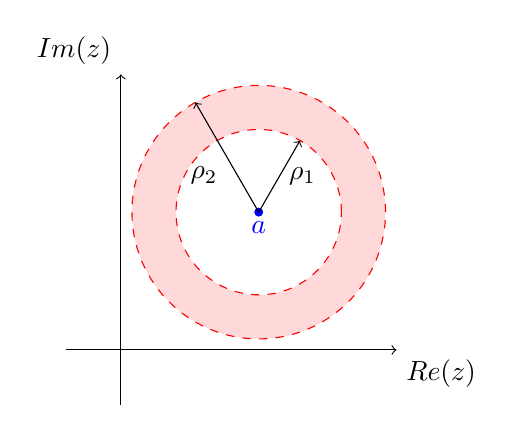
\begin{tikzpicture}[scale=0.7]
    % Ejes
    \draw[->] (-1,0) -- (5,0) node[below right] {$\operatorname{Re}(z)$};
    \draw[->] (0,-1) -- (0,5) node[above left] {$\operatorname{Im}(z)$};

    % Centro a
    \filldraw[blue] (2.5,2.5) circle (2pt) node[below] {$a$};

    % Región sombreada entre las dos circunferencias
    \fill[red!15, even odd rule] 
      (2.5,2.5) circle (2.3)
      (2.5,2.5) circle (1.5);

    % Contornos
    \draw[red, dashed] (2.5,2.5) circle (1.5);
    \draw[red, dashed] (2.5,2.5) circle (2.3);

    % Radio de la menor
    \draw[->] (2.5,2.5) -- ++(60:1.5)
      node[midway, right] {$\rho_1$};
    % Radio de la mayor
    \draw[->] (2.5,2.5) -- ++(120:2.3)
      node[midway, below left] {$\rho_2$};
  \end{tikzpicture}
  \caption{Corona en el plano complejo.}
  \label{fig:corona_complx}
\end{figure}

Veamos un ejemplo.
\begin{example}
  Determinar la región en el plano complejo definida por $\lvert z-3+i\rvert\leqslant4$.

  \textbf{Solución}: La desigualdad es válida precisamente para todos los $z$ cuya distancia a $a=3-i$ no es mayor que $4$. Por tanto, se trata de un disco circular cerrado de radio $4$ con centro en $3-i$.

  Gráficamente tenemos
  \begin{figure}[ht]
    \centering
    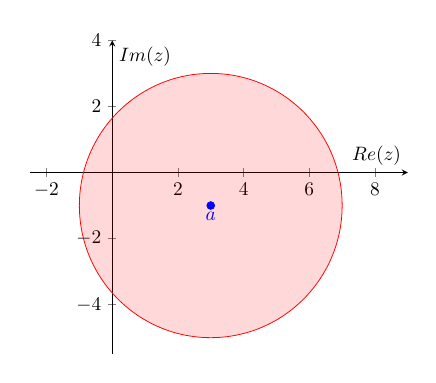
\begin{tikzpicture}[scale=0.7]
      \begin{axis}[
        axis lines = middle,
        xlabel = {$\operatorname{Re}(z)$},
        ylabel = {$\operatorname{Im}(z)$},
        xmin=-2.5, xmax=9,
        ymin=-5.5, ymax=4,
        ];
        \draw[red] (3,-1) circle (4);
        \fill[red, opacity=0.15] (3,-1) circle (4);
        \filldraw[blue] (3,-1) circle (2pt) node[below] {$a$};
      \end{axis}
    \end{tikzpicture}
  \end{figure}
\end{example}
